\section{\tool{} Leakage Definition}
\label{sec:trace-qif}
In this section, we discuss how \tool{} quantifies the amount of leaked
information. \tool{} adopts a dynamic-based approach to quantifying the leaked
information. We first present the limitation of existing quantification metrics.
After that, we introduce the abstract of our model and math notations for the
paper and propose our method.

\subsection{Problem Setting}
Existing static-based side-channel quantification
works~\cite{182946,Wichelmann:2018:MFF:3274694.3274741 } define information
leakage with max entropy or Shannon entropy. These definitions provide a strong
security guarantee when one tries to prove a program is secure.  If zero bit of
information leakage is reported, the program is secure. However, it is not
useful in practice if their tools report the program leaks some information.
Because their reported result is the ``average'' leakage, while in an attack
scenario, the leakage could be much severe.
%Moreover, those metrics does not apply to static method.


\begin{figure}[h!]
    \centering
    \begin{lstlisting}[xleftmargin=.03\textwidth,xrightmargin=.01\textwidth]
char key[9] = input();
if(strcmp(key, "password")){
    pass();     //branch 1
}else{
    fail();     //branch 2
}
\end{lstlisting}
    \caption{A dummy password checker}
    \label{fig:password-checker}
\end{figure}

We consider a dummy password checker shown in Figure~\ref{fig:password-checker}.
The password checker will take an 8-byte char array as the input and check if
the input is the correct password. If an attacker knows the code executes branch
$\{{1\}}$ by side-channel attacks, he can infer the password equals to
``password'', in which case the attacker can entirely retrieve the password.
Therefore, the total leaked information should be 64 bits, which equals to the
size of the sensitive input, when an attacker observes the code executes branch
$1$.

However, previous static-based approaches cannot precisely reflect the amount of
the leakage. According to the definition of Shannon entropy, the leakage will be
$\frac{1}{2^{64}}*\log_{2}\frac{1}{2^{64}} + \frac{2^{64}-1}{2^{64}}
*\log_{2}\frac{2^{64}-1}{2^{64}} \approx 0$ bits. Because the program has two
branches, tools based on max-entropy will report the code has $\log_2{2} = 1$
bit leakage.

Both approaches fail to tell how much information is leaked during the execution
precisely. The problem with existing methods is that they are static-based and,
the input values are neglected by their approaches. They assume an attacker runs
the program multiple times with many different or random sensitive inputs. As
shown in Figure~\ref{fig:gap}(a), previous models, both Shannon entropy and max
entropy, give an ``average'' estimate of the information leakage. However, it is
not the typical scenario for an adversary to launch a side-channel attack. When
a side-channel attack happens, the adversary wants to retrieve the sensitive
information, in which case the sensitive information is fixed (e.g., AES keys).
The adversary will run the attack over and over again and guess the value bit by
bit, as in Figure~\ref{fig:gap}(b). Like the previous example, the existing
static method does not work well in those situations. We want to produce a
theory for dynamic analysis that if the theory says an attack leaks $x$ bits of
secret information from a side-channel vulnerability, then $x$ should be useful
in estimating the sensitive level of the side-channel. However, the above
methods all fail in real attack models. This is the first challenge we face
\textbf{(Challenge C1)}.

\begin{figure}
    \centering
    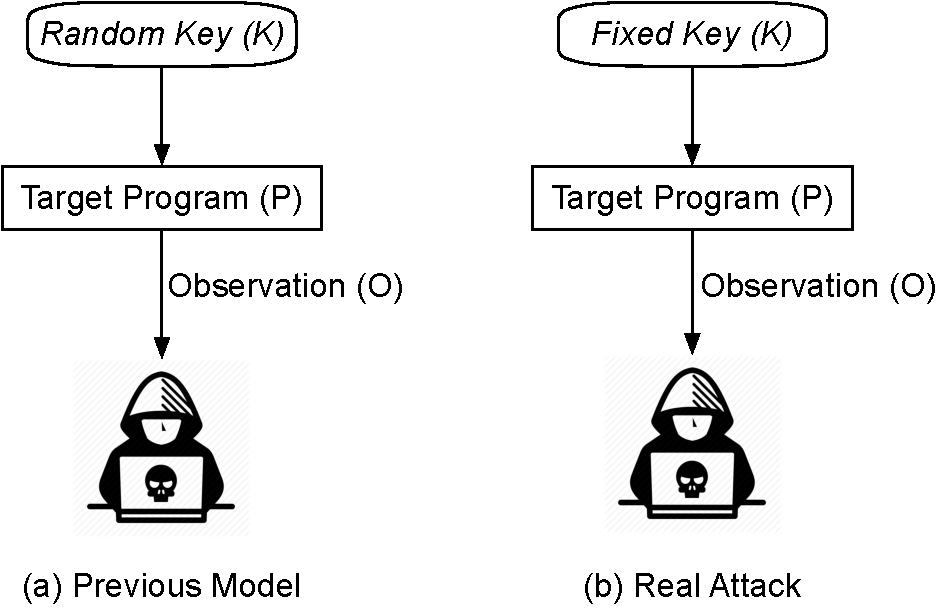
\includegraphics[width=.8\columnwidth]{./figures/RA.pdf}
    \caption{The gap between the real attack and previous model}\label{fig:gap}
\end{figure}


\subsection{Notations}
In the section, we give necessary definitions and notations for dealing with
programs and side-channels. We use capital letters (e.g., $A$) to represent a
set. $|A|$ represents the cardinality of the set $A$. We use corresponding lower case
letters to represent one element in the set (e.g., $a \in A$).

We assume a program ($\beta$) has $K$ as the sensitive input. $K$ should be a
finite set of keys. The program also takes known messages $M$ as the input. The
model applies to most cryptosystems. For example, during the AES encryption,
$\beta$ is the encryption function. $K$ is AES key, and $M$ is messages to be
encrypted. During the execution, an adversary may have some observations ($O$)
from the program. Examples of those observations include timing, CPU usages, and
Electromagnetic signals (EM). In this paper, we consider secret-dependent
control-flows and secret-dependent memory accesses as observations.

With the above definitions, we define the following mapping between $\beta$,
$K$, $M$, and $O$:

\begin{displaymath}
    \beta(K, M) \rightarrow O
\end{displaymath}

We model a side-channel with the following way. An adversary does not have
access to $K$, but he knows $\beta$, $M$, and $O$. For one execution of a
deterministic program, once $k \in K$ and $m \in M$ are fixed, the observation
($o \in O$) should also be determined. As an attacker, he knows $\beta$, $o$,
and $m$. The attacker wants to infer the value of $k$. We use $K^o$ to denote
the set of possible $k$ values that produce the same observation:

\begin{displaymath}
    K^o = \{ k \in K \, |\, \beta(k, m) \rightarrow o\}
\end{displaymath}

Then the problem of quantifying the amount of leaked information can be
transferred into the following question.
\emph{How much uncertainty of $K$ can be reduced if an attacker knows $\beta$, $m$, and $o$?}

\subsection{Theoretical Analysis \textbf{(Solution to Challege C1)}}
Now we present our metric to quantify the amount of leaked information from
dynamic analysis.

In information theory, the mutual information (MI) is a measure of the mutual
dependence between the two variables. Here we use MI to describe the information
dependence between $K$ and $O$, which is defined as:

\begin{equation} \label{eq:1}
    I(K;O) = \sum_{k {\in} K}{\sum_{o {\in} O}{p(k, o)\log_2\frac{p(k, o)}{p(k)p(o)}}}
\end{equation}

where $P(k_i, o_i)$ is the joint discrete distribution of $K$ and $O$.
Alternatively, the mutual information can also be equivalently expressed as:

\begin{equation} \label{eq:2}
    I(K;O) = H(K) - H(K|O)
\end{equation}

$H(K|O)$ is the entropy of $K$ with the condition $O$. It quantifies the
uncertainty of $K$ given the value of $O$. In other word, the conditional
entropy $H(K|O)$ marks the uncertainty about $K$ after an adversary has gained
some observations ($O$).
\begin{equation}
    H(K|O) = - \sum_{o {\in} O} {p(o) \sum_{k {\in} K}{p(k|o)\log_2p(k|o)}}
\end{equation}

In this project, we hope to give a very precise definition of information
leakages. Suppose an attacker runs the target program multiple times with one
fixed input, we want to know how much information he can infer by observing the
memory access patterns ($o$). We come to the simple slogan
~\cite{10.1007/978-3-642-00596-1_21} %% where the information
%% leakage equals:
%% \textbf{Initial uncertainty - remaining uncertainty}
that
\begin{align*}
     & \mathit{Information\ leakage} =                                         \\
     & ~~~~~~ \mathit{Initial\ uncertainty} - \mathit{Remaining\ uncertainty}.
\end{align*}

Now we compare Eq.~(\ref{eq:2}) with the above slogan, we find $H(K)$
is the $\mathit{Initial\ uncertainty}$ and $H(K|O)$ is $\mathit{Remaining\
uncertainty}$. During a real attack, the observation ($o$) is known.  We
have $H(K|O) = H(K|o)$.

Therefore, we define the amount of leaked information as
\begin{displaymath}
    Leakage = H(K;o) = H(K) - H(K|o)
\end{displaymath}

For a program ($\beta$) without knowing any domain information, all the sensitive
input should appear equally. Therefore, for any $k \in K$, $p(k) =
\frac{1}{|K|}$. So we have
$$H(K) = \sum_{k {\in} K}\frac{1}{|K|}\log_2{|K|} = \log_2{|K|}$$
For any $k' \in K \setminus K^o$, $p(k'|o) = 0$. We get
\begin{align*}
    H(K;o) & = - \sum_{k {\in} K^o}{p(k|o)\log_2p(k|o)}                         \\
           & \qquad   - \sum_{k` {\in} (K \setminus K^o)}{p(k'|o)\log_2p(k'|o)} \\
           & = \sum_{k {\in} K^o}\frac{1}{|K^o|}\log_2{|K^o|}                   \\
           & = \log_2{|K^o|}
\end{align*}


\begin{mydef}
    \label{def}
    Given a program $\beta$ with the input set $K$,
    an adversary has the observation $o$ when the input $k{\in}K^o$.
    We denote it as
    $$\beta(K^o, m) \rightarrow	o$$

    The leakage $L_{\beta(k)\rightarrow o}$ based on the observation ($o$) is
    $$L_{\beta(k)\rightarrow o} = \log_2{|K|} - \log_2{|K^o|}$$
\end{mydef}

With the new definition, if an attacker observes that the code in
Figure~\ref{fig:password-checker} runs the branch 1, then the $K^{o^{1}} =
\{\mathrm{``password"}\}$. Therefore, the information leakage $L_{P(k)=o^{1}} =
\log_2{2^{64}} - \log_2{1} = 64$ bits, which means the key is totally leaked. If
the attacker observes the code hits branch 2, the leaked information is
$L_{P(k)=o^{2}} = \log_2{2^{64}} - \log_2{(2^{64}-1)} \approx 0$ bit.


We can also calculate the leaked information from the sample code in
Figure~\ref{fig:side-channel}. As the size of input sensitive information is
usually public. The problem of quantifying the leaked information has been
transferred into the problem of estimating the size of input key $|K^o|$ under
the condition $o \in O$. The result is shown in Table~\ref{shtable2}. We can see
that some branches or traces leak much more information than some others. In
contrast, an \emph{average} estimate based on random secret input information of
1 or 2 bits, as shown in \S\ref{sec:background_leak} and Table~\ref{shtable}, is
not very useful in practice as an attacker is able to get much more leaked
information in some attack scenarios.

\begin{table}[ht]
    \centering
    \caption{New leakage modeling results}
    \label{shtable2}
    %  \resizebox{.8\columnwidth}{!}{
    \begin{tabular}{l|cccc}
        \hline
        %Observation (o)     & $\emptyset$ & ${\{1\}}$ & ${\{2\}}$ & ${\{1, 2\}}$ \\ \hline
        %Number of Solutions &  32876 & 20 & 32634 & 16 \\ \hline
        %Possibility (p)     & 0.5016 & 0.0003 & 0.4980  & 0.0002   \\
        Observation ($o$)         & $\emptyset$ & ${\{1\}}$ & ${\{2\}}$ & ${\{1, 2\}}$ \\ \hline
        Number of Solutions       & 32876       & 20        & 32634     & 16           \\ \hline
        Leaked Information (bits) & 1.0         & 11.7      & 1.0       & 12.0         \\
        \hline
    \end{tabular}
    %    }
\end{table}

\subsection{Our Conceptual Framework}
\label{side-channel:condition}
We now discuss how to model the observation (o), which is the direct information
that an adversary can get during the attack.

During the execution, a program ($\beta$) have many temporary values ($t_i \in
T$). Once $\beta$ (program), $k$ (secret), and $m$ (message, public) are
determined, $t_i$ is also fixed. Therefore, $ t_i = f_i(\beta, k, m)$, where $f_
i$ is a function that maps $t_i$ and ($\beta$, $k$, $m$).

In the paper, we consider two code patterns that can be exploited by an attacker,
\emph{secret-dependent control transfers} and \emph{secret-dependent data
accesses}. In other words, an adversary has observations based on control-flows
and data accesses.

\subsubsection{Secret-dependent Control Transfers}
We think a control-flow is secret-dependent if different input sensitive keys
($K$) can lead to different branch conditions. For a specific branch, the
condition is either true or false. Therefore, the branch condition is always a
boolean variable.

We think a branch is secret-dependent if:
$$\exists k_{i1}, k_{i2} \in K, \,f_i(\beta, k_{i1}, m) \neq f_i(\beta, k_{i2}, m)$$

An adversary can observe which branch the code executes, if the branch condition
equals to $t_b$. We use the constraint $c_i : f_i(\beta, k, m) = t_b$ to model
the observation on secret-dependent control-transfers.

\subsubsection{Secret-dependent Data Accesses}
Similar to secret-dependent control transfers, a data access operation is
secret-dependent if different input sensitive keys ($K$) can lead to different
memory addresses. We use the model from CacheD~\cite{203878}. The low $L$ bits
of the address are irrelevant in side-channels.

We consider a data access is secret-dependent if:
$$\exists k_{i1}, k_{i2} \in K, \,f_i(\beta, k_{i1}, m) >> L \neq f_i(\beta, k_{i2}, m) >> L$$

If the branch condition equals to $t_b$, we can use the constraint $c_i :
f_i(\beta, k, m) >> L = t_b >> L$ to model the observation on secret-dependent
control-transfers.

With the above definitions, we can model an attacker's observation with math
formulas. For example, in Figure~\ref{fig:side-channel}, if an attacker observes
the code executes the branch 1, we have $c_5: k_1 + k_2 < 8$ to describe an
attacker's knowledge and $K^{o5} = \{k_1,\, k_2\,|\, (k_1 + k_2) < 8\}$. If an
attacker observes the code executes the branch 2, we have $c_8: k_1 - k_2 > 0$
and $K^{o8} = \{k_1,\, k_2\,|\, (k_1 - k_2) > 0\}$.
